\documentclass{article}
\usepackage[utf8]{inputenc}
\usepackage[T1]{fontenc}
\usepackage{graphicx}
\usepackage{geometry}
\usepackage{xcolor}
\geometry{a4paper}
\geometry{top=2.5cm, bottom=2.5cm}
\title{User Manual for the Power Stablization Box}
\author{Xiaoyu Jiang}
\date{03/21/2018}
\begin{document}
\maketitle
%------------------------------------------------------------------------------------------------------------------------------------------------------------------------------------------------------------------------------------
\section{Introduction}

The Rotating-waveplate-based DC Noise Eater is a system designed to deal with slow power fluctuations of laser beams in experiments. The basic diagram of the feedback system can be shown as follow:

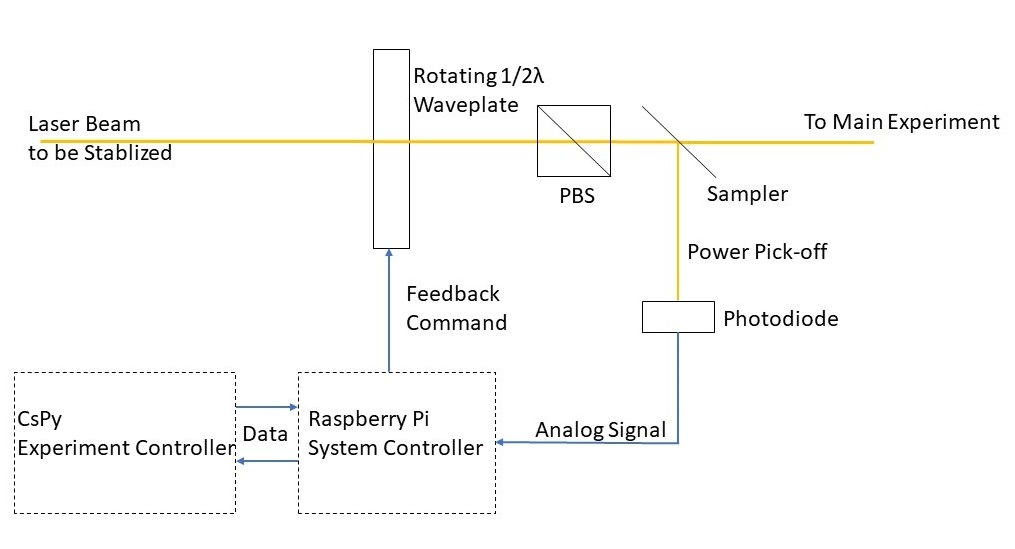
\includegraphics[height=3in]{noiseeaterdiagram.JPG}\newline
In this system, a linealy polarized laser beam goes through a $1/2\lambda$ mounted on a rotating stage. Then the power of the beam gets measured by a photodiode, and the measurement is sent to a Raspberry Pi(RPi). The RPi compares the measured laser power to the desinated value, calculates the feedback signal, and sends it to the rotating stage. The stage will rotate accordingly to change the polarization of the beam, which also changes the power of the beam that goes through the PBS. The loop will be executed repeatedly to eventually stablize the laser power to the setpoint. At the same time, the RPi can also be identified as a TCP/IP instrument on the CsPy experiment controller, which enables data exchange between them. CsPy can receive measurements from the RPi, and dynamically set experiment parameters. \newline\newline

\subsection{Hardware components}
A list of componets needed to setup the system:\newline\newline
\textbf{A RPi 2/3 board}\newline
The RPi act as the major controller/server\newline\newline
\textbf{A Waveshare High-Precision AD/DA board}\newline
The way that Rapsberry Pi interacts with other electronic devices is through its USB ports or the series of digital IO pins installed on board. This makes it unable to process or send analog signals directly. For this reason we are using this AD/DA shield in the system. It can be installed directly on top of the RPi, while it receives the data from its own analog port, convert it to a digital signal with the ADS1256 chip, and passes the digital information to RPi through the IO pins.  \newline\newline
\textbf{A 5V DC power suppy}\newline
Power supply for the RPi. Normally a 1A source is sufficient to keep the RPi working. But more current is needed if the rotation stage is driven directly by the RPi. Normally a power USB hub would be used to provide rotators with enough current to draw from.  \newline\newline
\textbf{Thorlabs K10CR1 rotation stage, at most 4 per RPi}\newline
\textbf{$1/2\lambda$ waveplates of according wavelengths, 1 per rotation stage}\newline
The rotator-waveplate combination enables intensity control. The number of rotators that can be driven by a single RPi is limited by 4, due to the reason that there are at maximum 4 differential analog input ports on the AD shield we are using. \newline\newline
\textbf{Pin housing connectors, wires and cables for connection}\newline
Except for driving rotators and recieving inputs from the shield, the RPi also needs to receive triggers and generate error signals. Both signals are connected directly to the general-purpose-input-output(GPIO) pins on the RPi.  \newline
The RPi also need to be connected to the internet/intranet through wire/wireless communications. \newline\newline
\textbf{(If necessary)A power USB hub}\newline
\textbf{(If necessary)A set of monitor, USB keyboard and USB mouse, for initially setting up the RPi}\newline
\textbf{(If necessary)A micro SD card providing memory for RPi}\newline
\textbf{(If necessary)Remote PC for dynamic interactions with the system}\newline\newline
To reduce the load of setting up various hardware components we have severl boxes already set up which would reduce the load of installing shields and connecting wires. Currently the boxes can be found in the undergraduate's office. 

\subsection{Software components}
Generally to make the system work, a user needs to run a main python program on RPi, with all the hardware components correctly connected and configured. Multiple libraries are used/self-written to enable communication between the main program and other hardware. We here give a brief introducion of the software structure of our system to illustrate the related programs/libraries.  \newline\newline
\textbf{Operation system for RPi}\newline
The operations system installed on the RPi is Raspibian, a Linux-like system that can be downloaded through RPi's official website. All the commands used in the follwing sections are general Linux orders and are based on this system. \newline
Please note that for compatibility purposes we are using verison 4.49 instead of the most up-to-date version of Raspibian. Users can always install the lasted version to initially set up and bump it back to 4.49 later.\newline\newline
\textbf{Main program}\newline
All the python codes are currently saved in the project's github page. There will be commands showing how to pull the repository to a new RPi in following sections. Once sucessfully done, one can always find the projects code under /home/pi/PowerStablizer/project1. \newline
The main code is named sx.y.py, where x.y is the version number. In the main program we initially set up the system, read the beam power measurements, use PID method to calculate the feedback signal, and drive the rotators to make adjustments. Triggering and error reporting are also processed in the program. It also provides sockets to communicate with CsPy. Generally users don't need to read every line of the main program, while they just need to know a certain set operations to change the settings of the system(which will also be covered below). However as the system is far from perfect, any suggestions about the code would be appreciated. \newline\newline
\textbf{Communicating with the rotation stage}\newline
The rotating stage we are using are Thorlabs K10CR1 rotation mount series. It can communicate with PCs through USB connection by using a C library, through serial commands by following the low-level communication protocol. Both documents can be found in git/wiki or are available in the official website. \newline
As the C libraries uses a set of dynamic-link-libraries(DLLs) which are only compatible in Windows, we choose to use the lower-level serial protocols to communicate with the rotators. A python library is already written by XJ that can cover all the basic operaitions on the rotator. The library is named Rotator and can be found under the Git repository. In most cases users don't need to read the code, for relevant operations are already included in the main program. But one can always look into it if related bug exists, or is willing to send more complicated commands to the rotator.\newline
A library named Devicesetup can also be found. While the library above focuses on communicating with the rotator in the correct form, this library helps RPi to identify connected devices and set up correct serial connections to them. Both libraries are used in the main program.\newline\newline
\textbf{Communicating with the AD shield}\newline
As introduced before the AD shield is used to read analog signals and convert them to be digital. The only connection between the shield and the RPi are through the 40 GPIO pins on RPi. The pins allows RPi not only to read digital data, but also to have full control of the shield by ordering it to start, stop or choose to read from a paticular analog differential input pot. To achieve these functionalities a library is used. The library is a non-official online version in Git, and was further edited by XJ. It is named Shield and can be found under the same repository. \newline
The official library comes with the shield is also written in C. So far I am still not able to use it in this system. \newline\newline
\textbf{Communicating with the GPIO pins}\newline
To communicate with the GPIO pins we are using the official library GPIO that comes with every new RPi. Online documents for GPIO can be easily found.\newline\newline
\textbf{Remote Desktop communication}\newline
One can use Putty, a remote desktop software, to login onto the RPi as a client via SSH. One can then start/end the program or change relevant parameters. This is only possible when RPi is connected to the net and password is known. \newline\newline

%------------------------------------------------------------------------------------------------------------------------------------------------------------------------------------------------------------------------------------
\section{Installation}
Before setting up the system, we need to initialize the components used in the system.
\subsection{Configure the Raspberry Pi}
%------------------------------------------------------------------------------------------------------------------
\textbf{Installing Operation System}: We are using Raspbian Jessie with desktop as operation systems on the RPis. A micro SD card and image writing tools are needed. The image file can be downloaded from https://www.raspberrypi.org/downloads/raspbian/. \newline\newline
\textbf{First Boot}: Once Raspbian is installed, the RPi is ready to be powered up. Connect the RPi to monitors via HDMI and to mouse and keyboard via USB, then turn on the power supply. \newline
During the first boot, some settings are needed, so that all the following operations can be done with SSH(Secure Shell).\newline\newline
Setting interfacing option: \newline Open the terminal window and type the following command: \newline
\textcolor{gray}{\$ sudo raspi-config} \newline
Then in 'Interfacing options', choose to enable SSH and SPI. \newline\newline
Identify IP address: \newline First have the RPi connected to the internect. For now we are using wireless network UWNet. Then in command window, use:\newline
\textcolor{gray}{\$ sudo ifconfig} \newline Next to the \textcolor{gray}{wlan0} entry you will see the IP address of the RPi, indicated by \textcolor{gray}{inet addr} \newline
Record the IP address.\newline\newline
%------------------------------------------------------------------------------------------------------------------
\textbf{Further Settings}: From here all other configurations can be done remotely with SSH. So all the following operations will be done in the command terminal.\newline\newline
Download wiringpi python package:\newline
Wiringpi is a package designed to make the communication between the RPi and its GPIO pins more convenient and effective. In command window, enter the following commands:\newline
\textcolor{gray}{\$ sudo apt-get install python-dev python-setuptools swig}\newline
\textcolor{gray}{\$ git clone –recursive https://github.com/WiringPi/WiringPi-Python.git}\newline
\textcolor{gray}{\$ cd WiringPi-Python}\newline
\textcolor{gray}{\$ git submodule update –init}\newline
\textcolor{gray}{\$ cd WiringPi}\newline
\textcolor{gray}{\$ sudo ./build}\newline
\textcolor{gray}{\$ cd ..}\newline
\textcolor{gray}{\$ swig 2.0 -python wiringpi.i}\newline
\textcolor{gray}{\$ sudo python setup.py install}\newline
Wiringpi package should be installed by now.\newline\newline
%------------------------------------------------------------------------------------------------------------------
Download the controller project:\newline
The controller project is  a python project developed by XJ to performs all the power stablizing fuctionality of the system. \newline
In terminal window enter the following commands:\newline
\textcolor{gray}{\$ git clone https://github.com/QuantumQuadrate/PowerStablizer}\newline
\textcolor{gray}{\$ mv /home/pi/PowerStablizer/project1 /home/pi}\newline
These commands downloads the repository from Github and moves the /project1 folder under /home/pi. This can be checked by whether or not one can successfully enter the project1 folder:\newline
\textcolor{gray}{\$ cd /home/pi/project1}\newline\newline
Bumping the system to version 4.49:\newline
The wiringpi python package has compatiblity problems with newest version of the firmware kernel, so we need to bump it to a more stable version:\newline
\textcolor{gray}{\$ sudo apt-get install rpi update}\newline
\textcolor{gray}{\$ sudo rpi-update 2ca627126e49c152beb1bf7abd7122ce076dcc65}\newline
Reboot the RPi after installation:\newline
\textcolor{gray}{\$ sudo reboot now}\newline
RPis can also be shut down remotely:\newline
\textcolor{gray}{\$ sudo shutdown now}\newline
%------------------------------------------------------------------------------------------------------------------
\subsection{Remote login via PuTTY}
Putty is a open source SSH software that can enable access to RPis remotely. For now we are using it as the communication tool in our project. \newline\newline
PuTTY can be downloaded freely from: http://www.putty.org/.\newline\newline
To use PuTTY for remote login, first switch on the power of the RPi. Then in configuration window of PuTTY, enter the IP address of the target RPi. Then enter 22 as Port and choose SSH as connection type. Click Open to start the session.\newline

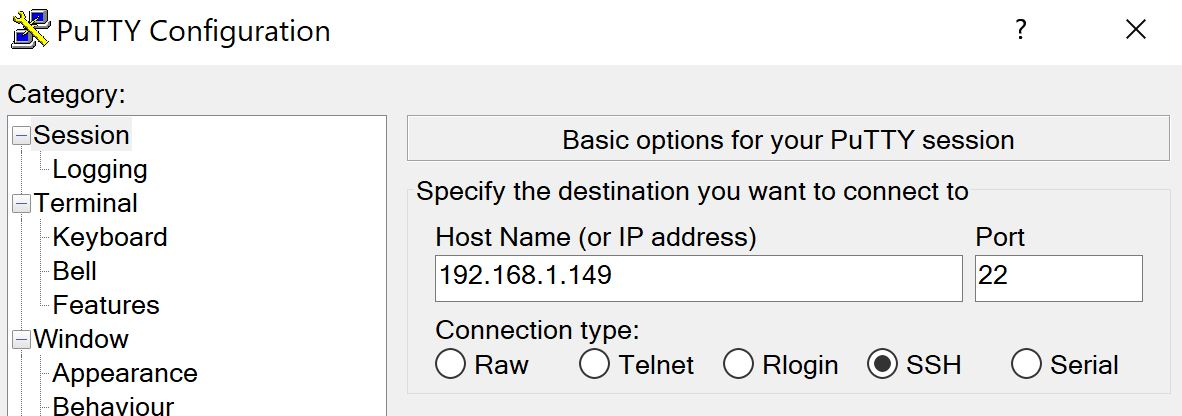
\includegraphics[height=1.5in]{putty1.JPG}\newline\newline
To login, user name and password are needed. A list of active RPis are being kept and updated on the wiki, so the username and passwords can be found in that document. \newline 
\subsection{Set up the analog shield and the box}
We use the Waveshare High Precision AD/DA Board as shield on the RPi to read analog inputs. \newline\newline
Before putting the shield into the box, remember to take off all the yellow jumpers on the shield with only two left: one across '5V' and 'Vcc', the other across '5V' and 'Vref'. The connection is shown as follow:\newline

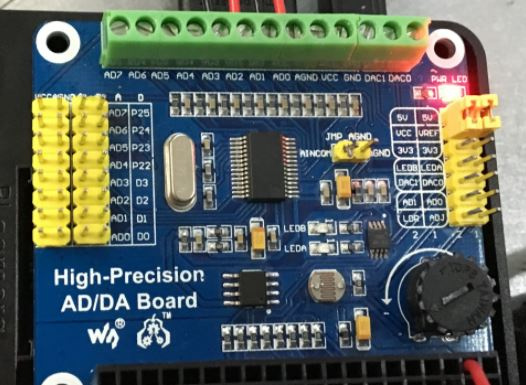
\includegraphics[height=2in]{rp1.JPG}\newline
The circuit diagram and front panel design of the box can be found on the wiki. Assemble the box according to the circuit diagram.
\subsection{Initialize the rotators}
We are using the Thorlabs K10CR1 rotating mounts as the unit to control the intensity of the laser beam.\newline\newline
The introduction, control software, C-language API and communication protocols can be found online\newline\newline
Before using the rotators in the experiments, please install Kinesis(motion control software) on a PC, have the device connected, and set the backlash parameter of the device to zero.\newline\newline
To achieve functionality of the system, a $1/2\lambda$ waveplate should be mounted in the rotator.
\subsection{Optical setup}
After 2.1-2.4 is done, one can start setting up the optical system as the basic diagram shows. 
%------------------------------------------------------------------------------------------------------------------
%------------------------------------------------------------------------------------------------------------------------------------------------------------------------------------------------------------------------------------
\section{Introduction to the box}
The front panel of each box looks like the following:

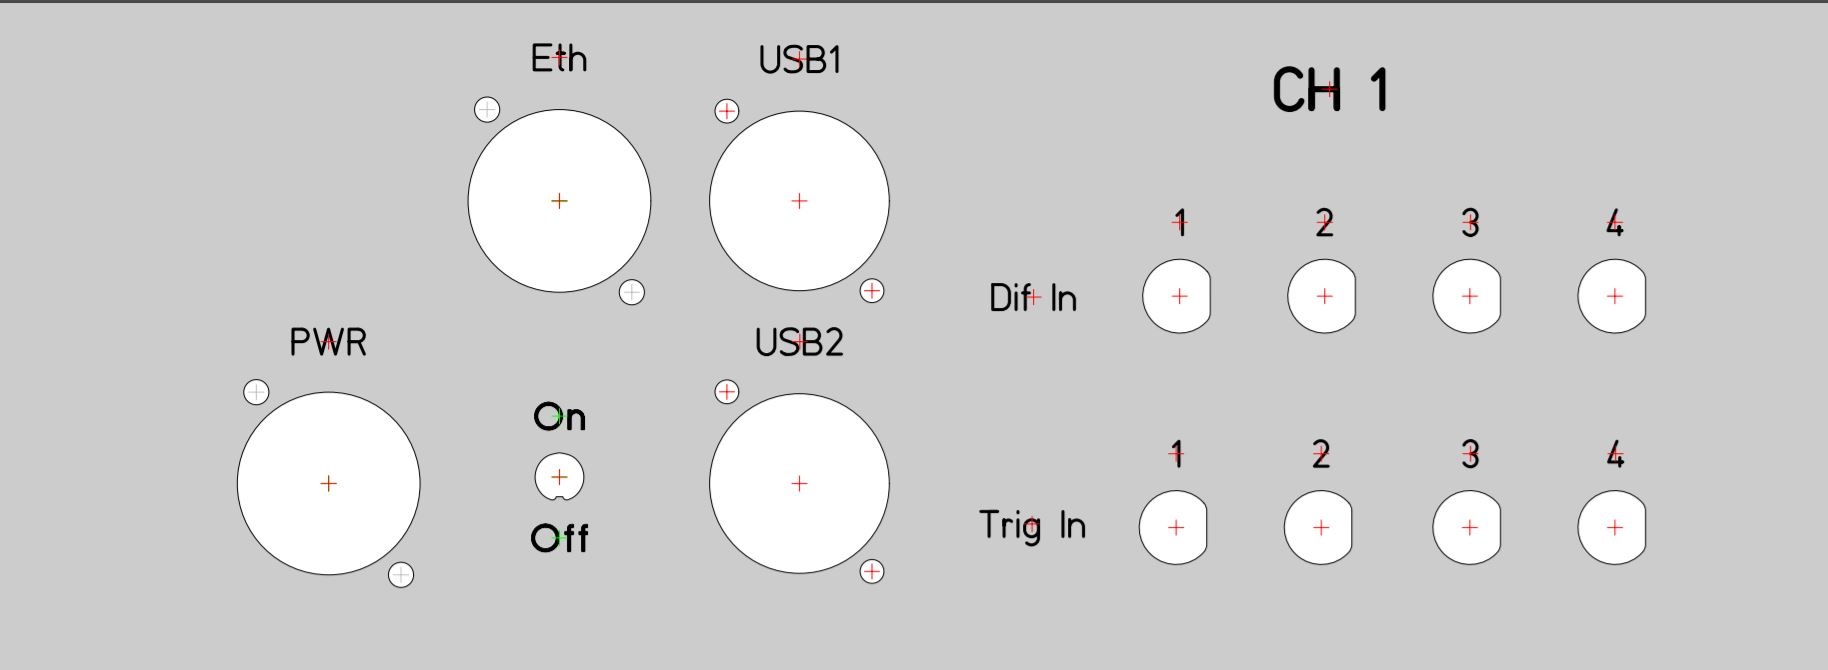
\includegraphics[height=2in]{box1.JPG}\newline
For each RPi, there are 2 USB ports, 4 analog inputs(Diff In), 4 digital inputs/outputs(Trig In), and 1 ethernet port on the box connected to it.

\subsection{USB ports}

There are 2 USB ports for each RPi in the box, labeled by 1 and 2. USB devices can be connected to the RPi through these ports. However the port name of the connected device inside the RPi is randomly assigned. One can check the port by entering:\newline
\textcolor{gray}{\$ ls /dev/ttyUSB*}\newline
Generally when connecting multiple K10CR1 rotators to the box, we normally don't connect them directly to the USB ports, for the RPi is not able to provide enough current to drive multiple motors. Instead, we should plug them into a self-powered USB hub, and then plug the hub into one of the USB ports. The number of rotators should not exceed 4, and the hub itself should be able to provide enough current for each K10CR1.\newline
\subsection{Input/Output}
The 4 analog inputs('Diff In') are labeled as 1-4 on the box. All of them are connected to the analog shield(Waveshare High Precision AD/DA Board) on the RPi.  Input $i$ is connected to AD$2i-2$ and AD$2i-1$ on the shield as a differential input. Generally we are using these ports to read analog voltage inputs from the photodiode, which is proportional to the intensity of the laser beam.\newline

The 4 digital input/ourputs('Trig In') are also labeled as 1-4 on the box. Each of the Diff In inputs are connected directly to two GPIO(general purpose input and output) pins on the RPi. The ground of the input signal are all connected to Pin 6 on the RPi, and the signals from port 1-4 are hooked to Pin 3,5,7,8 respectively. Generally we use these ports to receive the triggers from the experiment controller.\newline

The 'Trig In' signals are independent of the ‘Diff In' signals. One can have multiple rotators sharing the same trigger.\newline

On Raspberry Pi, all GPIO banks are supplied from 3.3V. Connection of a GPIO to a voltage higher than 3.3V will likely destroy the GPIO block.\newline

In principle the GPIO pins on a RPi are all digital ones, so we cannot send/receive analog signals directly to/from a RPi. As introduced before, an AD/DA shield can be used to realize these fuctions. It's also useful to note that the GPIO pins can be set to output a pulse-width modulated(PWM) signal, which can be converted to analog outputs with some external circuitry. 
\section{Running Stablization}
Remote login to the RPi, then enter the following path:\newline
\textcolor{gray}{\$ cd /home/pi/project1}\newline
\subsection{Start the program}
Use command:\newline
\textcolor{gray}{\$ sudo python s3.0.py}\newline
\subsection{Change stablization parameters}
In the main program, a lot of parameters can be set to fit the system into the main experiment. Most of the parameters are arrays with length of 4. This is because we have 4 'Diff In' channels on the box panel, and each of those channels correspond to a particular laser beam and a specific rotator. The parameter for each laser-stablization system should be different, so we have many 4-component arrays to set up each channels individualy.\newline


Use the following command to remote-edit the program and change parameters:\newline
\textcolor{gray}{\$ nano s3.0.py}\newline
The following parameters can be set: \newline\newline
(bool)\textbf{enable}: 1 for using,0 for not using the channel.Here the channels refer to the 'Diff In' ports on the box panel:\newline
enable=[1,1,1,1]\newline\newline
(string)\textbf{SN}: Serial number for the rotator connected to each channel, if in use:\newline
SN=['55000491','55000389','55000392','55000604']\newline\newline
(int/volts)\textbf{target}: Stablization target for the beam in each channel, if in use:\newline
target=[3,3,3,3]\newline\newline
(float)\textbf{KP}: Proportional part of feedback parameters for each channel:\newline
KP=[1,1,1,1]\newline\newline
(float)\textbf{KI}: Integral part of feedback parameters  for each channel(cannot be used for now, the new version is still being tested):\newline
KI=[0,0,0,0]\newline\newline
(int)\textbf{triglist}: For the specific 'Diff In' channel, specify which trig port it is using(please note that 0,1,2,3 in triglist corresponds to trigger channel 1,2,3,4 on the box):\newline
triglist=[0,0,0,0]\newline\newline
(float/seconds)\textbf{delaytime}: Set the time delay after trigger before measurement for each channel:\newline
delaytime=[0,0,0,0]\newline\newline
(float)\textbf{tintegral}: Set the time duration for measurements  in each channel. Multiple measurements will be done within this time limit and the average will be used for feedback:\newline
tintegral=[0.01,0.01,0.01,0.01]\newline\newline
(int)\textbf{integralwindow}: Set the length of the integral window in feedback calculation for each channel(cannot be used for now, the new version is still being tested):\newline
integralwindow=[10,10,10,10]\newline\newline
(bool)\textbf{readonly}: 1 for only reading out the signal,0 for running stablization:\newline
readonly=0\newline\newline
(bool)\textbf{enablebuffer}: 1 for enabling the input buffer(increase input inpedance),0 for disable:\newline
enablebuffer=0\newline\newline
%------------------------------------------------------------------------------------------------------------------
%------------------------------------------------------------------------------------------------------------------------------------------------------------------------------------------------------------------------------------
\end{document}

